%UTILE ? ajouter methi-ode au hasard mais avec bon deo-placement pourdiminuer SL(C) si possible !!!

\documentclass[a4,11pt]{article}
	\usepackage{template/css-color}
    \usepackage{template/css-gray}

    \usepackage{template/general}
    \usepackage{template/quote}
    \usepackage{template/algo}
    \usepackage{template/math}
    
    \usepackage[
        type={CC},
        modifier={by-nc-sa},
        version={4.0},
    ]{doclicense}
   

	\usepackage{tikz}
	\usetikzlibrary{trees}

% WATERMARK
	\usepackage[printwatermark]{xwatermark}


% DRAFT MODE !
%	\newwatermark[%
%		allpages,%
%		color=red!20,%
%		angle=45,%
%		scale=1.1,%
%		xpos=-10, ypos=30]{Z! - BROUILLON - TEXTE NON SÛR - Z!}
%
%	\newwatermark[%
%		allpages,%
%		color=red!20,%
%		angle=45,%
%		scale=1.1,%
%		xpos=5, ypos=-5]{PRÉSENCE PROBABLE DE GROSSES ERREURS}


%% NEED TO BE READ BY OTHERS !
%	\newwatermark[%
%		allpages,%
%		color=red!20,%
%		angle=45,%
%		scale=1.1,%
%		xpos=-10, ypos=30]{PRÉVERSION - TEXTE EN DEVENIR}
%
%	\newwatermark[%
%		allpages,%
%		color=red!20,%
%		angle=45,%
%		scale=1.1,%
%		xpos=5, ypos=-5]{BESOIN DE RELECTURES EXTERNES}


\begin{document}

\addtitle{%
    title      = {Baseball des couleurs - Une petite étude théorique},
    name       = {Christophe BAL},
    mail       = {projetmbc@gmail.com},
    version    = {Version du 2017-02-12},
    addlicence = yes,
%    repo       = {https://github.com/bc-writings-algo-general/algorithms_with_paper},
%    repofolder = {fr}
}

\vspace{3cm}

\hrule

\tableofcontents

\vspace{4ex}

\hrule

\newpage



\section{Origine du jeu}    % RELU. OK !
    L'auteur de ces modestes lignes a pris connaissance du jeu \quote{le baseball des couleurs} le jeudi 5 janvier 2017 lors d'une formation d'\quote{Informatique Débranchée} proposée par l'Académie de Grenoble. Ce jeu est inspiré du \quote{jeu de l’orange} proposé dans le livre \quote{L’informatique sans ordinateur - Programme d’activités d’éveil pour les élèves à partir de l’école primaire} de Tim Bell, Ian H. Witten et Mike Fellows qui a été adapté à l’utilisation en classe par Robyn Adams et Jane McKenzie (Septembre 2009 - 2e éd. juin 2014)
\footnote{
    Voir \url{http://csunplugged.org/books/}.
}.



\section{Les règles}    % RELU. OK !
    On considère cinq îlots colorés différemment que nous nommerons \quote{bases}. Chacune de ces bases contient deux trous pour y accueillir deux jetons.
Pour chaque couleur $\cal C$ sauf une, disons $\cal C^{\prime\prime}$, on a deux jetons de couleur $\cal C$.
Par contre, on a juste un jeton de couleur $\cal C^{\prime\prime}$.
La partie commence en mettant au hasard deux jetons sur chaque base sauf une qui ne contiendra qu'un seul jeton.
Voici un exemple où c'est le jeton noir qui est seul, et c'est sur la base bleue qu'il n'y a qu'un seul jeton.

\begin{center}   % [3, 1, 2, None, 3, 1, 4, 0, 4, 2]
    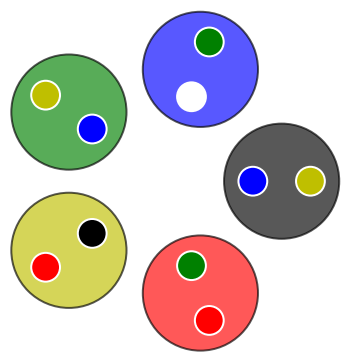
\includegraphics[scale= 0.3]{content/rules/start.png}
\end{center}

Le seul mouvement autorisé est le déplacement d'un jeton vers le trou libre à condition que le dit jeton et le trou soient dans des bases \quote{directement} voisines. Dans l'exemple ci-dessus, on ne peut donc bouger que l'un des jetons des bases bleue et rouge. Le but du jeu est d'obtenir la configuration suivante où chaque jeton a retrouvé sa base (la position du trou dans la base noire est sans importance).

\begin{center}
    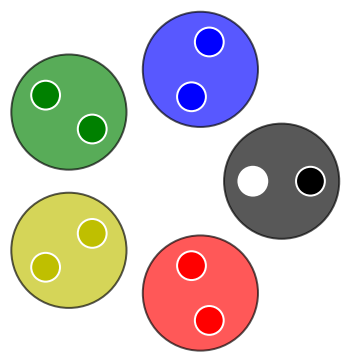
\includegraphics[scale= 0.3]{content/rules/end.png}
\end{center}

Si vous ne connaissez pas ce jeu nous vous conseillons, avant de lire la suite de ce document, d'essayer de trouver une méthode (il en existe plusieurs possibles et peut-être que vous trouverez d'autres points de vue que ceux que nous proposerons plus bas). Pour cela, il suffit d'expérimenter en vous fabriquant des bases et des jetons carrés, ce qui est très vite fait.


\paragraph{Remarque :} \hspace{-1em} dans ce jeu nous avons à tout moment accès à toutes les informations mais on pourrait très bien imaginer n'avoir accès qu'aux informations présentes sur trois bases voisines (concrètement, on mettrait les bases sur un plateau tournant avec au-dessus un cache ne laissant apparaître que trois bases). Il faut savoir qu'en informatique l'on peut avoir ce type de contrainte : par exemple, les routeurs qui dirigent les informations sur le réseau physique de l'internet n'ont pas une connaissance globale du réseau et pourtant ils arrivent à trouver d'assez bonnes solutions pour acheminer des données.



\section{Premier contact : la méthode \textit{\og une base à la fois \fg}}    % RELU. OK !
    Avant de chercher une solution optimale, commençons déjà par en trouver au moins une qui fonctionne
\footnote{
	Les problèmes d'optimisation d'algorithme se traitent toujours dans un second temps. Cette règle s'applique aussi constamment lorsque l'on programme.
}.
Laissant de côté le problème de la solution la plus efficace, nous avons assez vite les deux idées simples suivantes.

\begin{enumerate}
	\item Casser le cercle pour représenter les bases en ligne comme ci-dessous où il est important de bien mettre à gauche la base noire, celle n'ayant qu'un seul jeton de même couleur une fois le problème résolu.

	\item S'interdire tout mouvement de la base rouge, la plus à droite, à la base noire, la plus à gauche.
\end{enumerate}

\vspace{-0.4em}
\begin{center}   % [1, 2, 3, None, 4, 1, 4, 0, 2, 3]
	\includegraphics[scale= 0.45]{content/algo_selection/example/000.png}
\end{center}
\vspace{-0.8em}


L'ajout d'une contrainte va nous permettre de donner un algorithme simple à décrire mais aussi facile à valider. Par contre, nous devinons bien que nous nous interdisons de résoudre rapidement le problème.
%(les deux sections suivantes vont s'intéresser à la recherche d'une solution optimale)
La méthode que nous allons présenter va consister à remplir la cinquième base, puis la quatrième... en cherchant juste à rapatrier les jetons manquants. Voici des premiers mouvements possibles où vous noterez au passage qu'une fois une base remplie à droite, celle-ci n'est plus jamais utilisée (les étapes évoluent dans la colonne de gauche puis dans celle de droite).


\medskip

\begin{multicols}{2}
	\begin{center}   % [1, 2, 3, None, 4, 1, 4, 0, 2, 3]
		\includegraphics[scale= 0.45]{content/algo_selection/example/000.png}

		\includegraphics[scale= 0.45]{content/algo_selection/example/001.png}

		
\includegraphics[scale= 0.45]{content/algo_selection/example/002.png}

		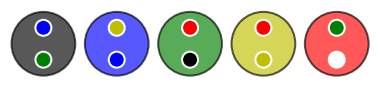
\includegraphics[scale= 0.45]{content/algo_selection/example/003.png}
		
		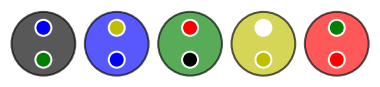
\includegraphics[scale= 0.45]{content/algo_selection/example/004.png}

		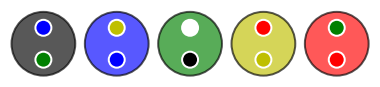
\includegraphics[scale= 0.45]{content/algo_selection/example/005.png}

		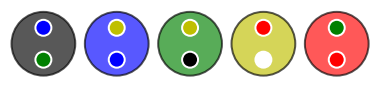
\includegraphics[scale= 0.45]{content/algo_selection/example/006.png}

		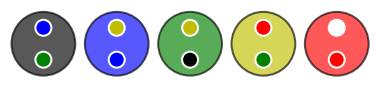
\includegraphics[scale= 0.45]{content/algo_selection/example/007.png}
	\end{center}
		
	\columnbreak
	\begin{center}
		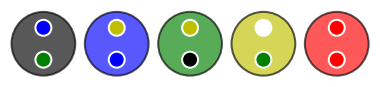
\includegraphics[scale= 0.45]{content/algo_selection/example/008.png}
		
		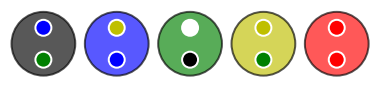
\includegraphics[scale= 0.45]{content/algo_selection/example/009.png}

		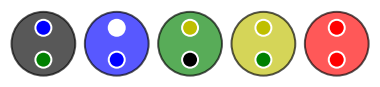
\includegraphics[scale= 0.45]{content/algo_selection/example/010.png}

		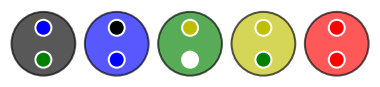
\includegraphics[scale= 0.45]{content/algo_selection/example/011.png}

		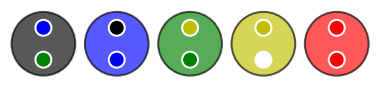
\includegraphics[scale= 0.45]{content/algo_selection/example/012.png}

		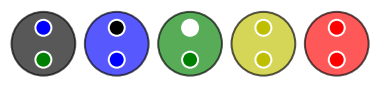
\includegraphics[scale= 0.45]{content/algo_selection/example/013.png}

		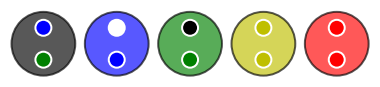
\includegraphics[scale= 0.45]{content/algo_selection/example/014.png}
			
		\textbf{\vdots}
		
		\textbf{etc}
	\end{center}
\end{multicols}


\medskip

Pour définir précisément comment fonctionne notre méthode, nous le faisons via l'algorithme suivant (l'écriture formelle employée est simple à comprendre).

\bigskip

\begin{algo}
	\Data{une configuration en ligne quelconque de début de jeu}
	\Result{une configuration en ligne où tous les jetons sont rentrées dans leur base}
	\vspace{0.4em}
    \Begin{
    	\vspace{0.4em}
		Aucune base n'est isolée pour le moment (nous allons vite voir ce que cela signifie).
    	\\
		\vspace{0.4em}
		\While{la configuration contient un jeton qui n'est pas dans sa base}{
			\vspace{0.4em}
			$\cal D$ : la base non remplie la plus à droite.
			\\
			$Coul_{\cal D}$ : la couleur de la base $\cal D$.
			\\
			\vspace{0.4em}
			\tcp{Les deux jetons de couleur $Coul_{\cal D}$ peuvent être dans la même base.}
			$j$ : un jeton de couleur $Coul_{\cal D}$ le plus à droite possible en dehors de la base $\cal D$. 
			\\
			$\cal J$ : la base du jeton $j$.
			\\
			\vspace{0.4em}
			\tcp{Deux contraintes.}
			$Ctr_1$ : ne pas passer par d'éventuelles bases isolées.
			\\
			$Ctr_2$ : ne pas bouger l'autre jeton de couleur $Coul_{\cal D}$ excepté si les deux jetons sont dans la même base.
			\\
			\vspace{0.4em}
			En respectant les deux contraintes $Ctr_1$ et $Ctr_2$,
			\\
			{\quad \textbullet} si besoin, amener le trou dans la base à droite de la base $\cal J$,
			\\
			{\quad \textbullet} puis utiliser le trou pour amener $j$ dans la base $\cal D$.
			\\
			\vspace{0.4em}
			\If{la base $\cal D$ est complète}{
				\vspace{0.4em}
				Isoler la base $\cal D$ (en la décalant un peu plus à droite par exemple). 
			}
        }
    }
\end{algo}

\bigskip

Nous devons vérifier la validité de cet algorithme c'est à dire vérifier trois choses.

\begin{enumerate}
	\item \textbf{\textsc{Non Ambiguïté :}} les actions proposées doivent être sans ambiguïté.

	\item \textbf{\textsc{Finitude :}} les actions à faire seront toujours en nombre fini.

	\item \textbf{\textsc{Résolution :}} une fois toutes les actions effectuées, nous devons obtenir une configuration où tous les jetons sont rentrées dans leur base.
\end{enumerate}


Le contrat de \quote{non ambiguïté} est rempli même si une certaine liberté est laissée pour déplacer le trou ou le jeton 
\footnote{
	Nous avons ici un bel exemple d'algorithme \quote{non déterministe} en ce sens qu'en lançant l'algorithme plusieurs fois sur la même configuration initiale, on ne passera pas forcément par les mêmes étapes intermédiaires pour résoudre le jeu.
}
à condition de ne pas visiter d'éventuelles bases isolées et sans bouger un éventuel jeton déjà bien placé dans la base la plus à droite non encore complète.
En pratique, la \quote{non ambiguïté} n'est jamais justifiée, par contre les deux derniers points doivent toujours faire l'objet d'une  démonstration comme nous allons le faire tout de suite.

\begin{proof}
	La preuve va s'appuyer sur deux résultats très simples dont on va donner des énoncés un peu formels mais avec des preuves visuelles très simples.


	\medskip

	\textit{Fait n°1 : on peut toujours déplacer le trou de la base où il est vers une base voisine $\cal V$ en laissant fixe un jeton de son choix dans la base $\cal V$.} 

	
	\medskip

	En effet, considérons le cas suivant où l'on veut déplacer le trou vers la troisième base en ne touchant pas au jeton rouge (les choix faits ne nuisent pas à la généralité du raisonnement pour un déplacement vers la droite).

	\vspace{-0.4em}
	\begin{center}   % [1, 2, 3, None, 4, 1, 4, 0, 2, 3]
		\includegraphics[scale= 0.45]{content/algo_selection/fact_1/000.png}
	\end{center}
	\vspace{-0.8em}

	Il suffit de procéder comme suit (c'est évident).

	\vspace{-0.4em}
	\begin{center}   % [2, 2, 3, None, 3, 1, 4, 0, 4, 1]
		\includegraphics[scale= 0.45]{content/algo_selection/fact_1/001.png}
	\end{center}
	\vspace{-0.8em}

	Le cas où la base voisine est à gauche se traite de façon analogue (on peut aussi utiliser un argument de type \quote{symétrie}).


	\medskip

	\textit{Fait n°2 : avec les notations de l'algorithme, on suppose le trou être dans la base ${\cal J}_d$ à droite de la base $\cal J$ du jeton $j$ à déplacer, et que cette base ${\cal J}_d$ n'est pas la base $\cal D$ à remplir. Dans ce cas, on peut placer le jeton $j$ dans la base ${\cal J}_d$ et le trou dans la base à droite de ${\cal J}_d$ en choisissant la place du trou.}

	
	\medskip

	La preuve est bien plus simple à comprendre que l'affreux énoncé ci-dessus (on se demande bien qui a pu rédiger un truc pareil). Ci-dessous, le jeton à déplacer est le jaune dans la deuxième base bleue, et nous choisissons de ne pas toucher au jeton jaune de la quatrième base jaune (le lecteur notera la généralité de la méthode proposée).

	\vspace{-0.4em}
	\begin{center}   % [1, 2, 3, 1, None, 0, 3, 2, 4, 4]
		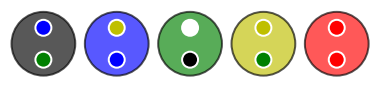
\includegraphics[scale= 0.45]{content/algo_selection/fact_2/000.png}

		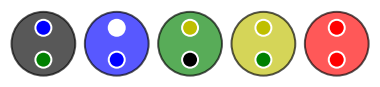
\includegraphics[scale= 0.45]{content/algo_selection/fact_2/001.png}

		
\includegraphics[scale= 0.45]{content/algo_selection/fact_2/002.png}

		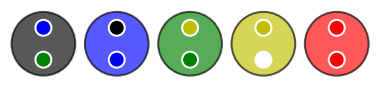
\includegraphics[scale= 0.45]{content/algo_selection/fact_2/003.png}

	\end{center}

	\vspace{-0.8em}


	\medskip

	\textit{Finitude et résolution} : commençons pas démontrer que l'algorithme commence par remplir la base rouge la plus à droite.


	\medskip

	Si la base rouge est déjà remplie, aucune action n'est requise et le résultat est vrai.
	Supposons donc que nous ayons au moins un jeton rouge dans l'une des quatre premières bases. Nous pouvons alors suivre les instructions de l'algorithme comme suit.


	\medskip

	\begin{itemize}
		\item[\textbullet] Grâce au fait n°1, il est effectivement possible de placer le trou dans la base à droite de celle du jeton rouge à déplacer, et ceci sans faire bouger un éventuel jeton rouge déjà dans la base rouge.

		\medskip

		\item[\textbullet] Ensuite, le fait n°2 nous permet d'amener le jeton rouge à déplacer dans l'avant-dernière base jaune et le trou dans la base rouge, de nouveau sans faire bouger un éventuel jeton rouge déjà dans la base rouge.

		\medskip

		\item[\textbullet] Il ne reste plus qu'à déplacer notre jeton rouge à la place du trou.
	\end{itemize}


	\medskip

	Si avant de faire ces opérations la base rouge contenait déjà un jeton rouge, nous avons rempli cette base, sinon l'algorithme nous fera remplir cette base dans un second temps (lors de la prochaine boucle \verb+Tant Que+).


	\medskip

	Une fois la base rouge remplie, celle-ci est isolée. Ceci implique que l'algorithme va travailler sur une version à quatre bases du jeu. Pour conclure, il suffit de reprendre le raisonnement ci-dessus non plus avec la base rouge mais avec la base jaune. Puis ensuite l'algorithme travaillera avec trois puis enfin deux bases et l'on raisonnera à chaque fois de la même façon. Ceci achève de montrer les propriétés de finitude et de résolution.

\end{proof}


\paragraph{Remarque :} \hspace{-1em} vous noterez que la démonstration précédente est valable pour un nombre quelconque $n \geqslant 2$ de bases (les plus tatillons pourront faire un raisonnement par récurrence).



\section{Soyons opportuniste : la méthode \textit{\og on avance au mieux \fg}}    % RELU. OK !
    La très grosse maladresse de la méthode \quote{une base à la fois} est de ne pas chercher à profiter de chaque déplacement du trou pour arranger la situation. Nous allons juste considérer cette idée pour proposer une nouvelle méthode de résolution
\footnote{
	Cette méthode a été proposée par les personnes en charge de la formation d'\quote{Informatique Débranchée} proposée par l'Académie de Grenoble le jeudi 5 janvier 2017. Voir la section \quote{Origine du jeu}.
}
qui elle aussi commence par mettre les bases en ligne de la base noire vers la rouge, et interdit tout mouvement de la base rouge à la base noire.

\begin{enumerate}
	\item On ordonne les couleurs, pour cela nous dirons que lorsque l'on va de la gauche vers la droite, on passe de couleurs froides à des couleurs chaudes.

	\item On commence par déplacer le trou vers la base rouge la plus chaude. Lors de ce déplacement, il faut déplacer à chaque fois le jeton le plus froid vers la gauche. Si les deux jetons de la base où va aller le trou sont de même chaleur, on choisit au hasard l'un des deux jetons.

	\item Une fois arrivé à la base rouge, on bouge le trou vers la base noire la plus froide. Lors de ce déplacement, ce sont les jetons les plus chauds qui migrent vers la droite. Si l'on tombe sur deux jetons de même chaleur, on applique la même tactique que ci-dessus.
	
	\item On continue les deux opérations $2$ et $3$ tant que toutes les bases ne sont pas complètes.
\end{enumerate}


Voici le début de l'application de cette méthode.

\medskip

\begin{multicols}{2}
	\begin{center}   % [1, 2, 3, None, 4, 1, 4, 0, 2, 3]
		\includegraphics[scale= 0.45]{content/algo_bubble/example/000.png}

		\includegraphics[scale= 0.45]{content/algo_bubble/example/001.png}

		
\includegraphics[scale= 0.45]{content/algo_bubble/example/002.png}

		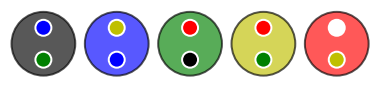
\includegraphics[scale= 0.45]{content/algo_bubble/example/003.png}

		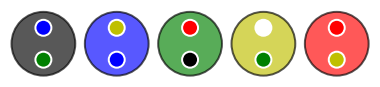
\includegraphics[scale= 0.45]{content/algo_bubble/example/004.png}

		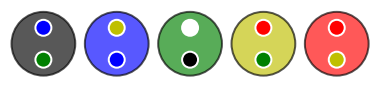
\includegraphics[scale= 0.45]{content/algo_bubble/example/005.png}

		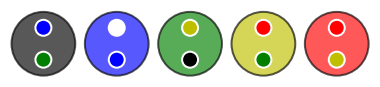
\includegraphics[scale= 0.45]{content/algo_bubble/example/006.png}

		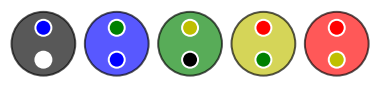
\includegraphics[scale= 0.45]{content/algo_bubble/example/007.png}
	\end{center}
	
	\columnbreak
	
	\begin{center}
		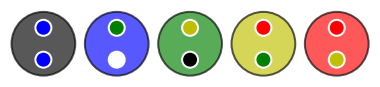
\includegraphics[scale= 0.45]{content/algo_bubble/example/008.png}

		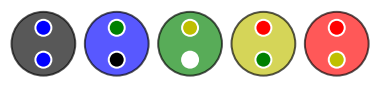
\includegraphics[scale= 0.45]{content/algo_bubble/example/009.png}

		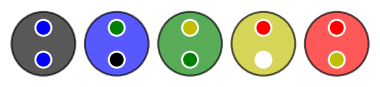
\includegraphics[scale= 0.45]{content/algo_bubble/example/010.png}

		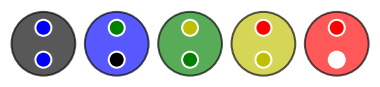
\includegraphics[scale= 0.45]{content/algo_bubble/example/011.png}

		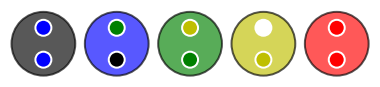
\includegraphics[scale= 0.45]{content/algo_bubble/example/012.png}

		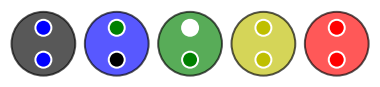
\includegraphics[scale= 0.45]{content/algo_bubble/example/013.png}

		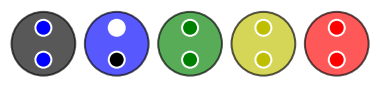
\includegraphics[scale= 0.45]{content/algo_bubble/example/014.png}
		
		\textbf{\vdots}

		\textbf{etc}
	\end{center}
\end{multicols}


Intuitivement, on sent bien que l'on ne va pas entrer dans une boucle infinie mais encore faut-il passer de l'intuition à une preuve irréfutable. Pour cela donnons d'abord une version plus formelle de notre nouvel algorithme de résolution (pour ordonner les couleurs nous allons les numéroter afin de simplifier les explications tout en raisonnant de façon très générale).

\bigskip

\begin{algo}
	\Data{une configuration en ligne quelconque de début de jeu}
	\Result{une configuration en ligne où tous les jetons sont rentrées dans leur base}
	\vspace{0.4em}
    \Begin{
		\vspace{0.4em}
    	On numérote de $0$ à $4$ les bases de la gauche vers la droite.
		\\
		On associe chaque couleur au numéro de la base de la dite couleur.
		\\
		\vspace{0.4em}
		\tcp{d donne la direction que doit suivre le trou.}
		\tcp{\quad \textbullet{} d = 1  pour un déplacement vers la droite.}
		\tcp{\quad \textbullet{} d = -1 pour un déplacement vers la gauche.}
		$d \leftarrow 1$
		\\
		\vspace{0.4em}
		\While{la configuration contient un jeton qui n'est pas dans sa base}{
			\vspace{0.4em}
			$t$ : numéro de la base où est le trou.
			\\
			\vspace{0.4em}
			\uIf{$(d \, , t) = (1 \, , 4)$}{
				\vspace{0.4em}
				$d \leftarrow (-1)$
				\\
				\vspace{0.4em}
			}
			\uElseIf{$(d \, , t) = (-1 \, , 0)$}{
				\vspace{0.4em}
				$d \leftarrow 1$
				\\
				\vspace{0.4em}
			}
			\Else{
				\vspace{0.4em}
				\tcp{v est le numéro de la base voisine de celle du trou où l'on doit mettre ce dernier.}
				$v \leftarrow t + d$
				\\
				\vspace{0.4em}
				\uIf{d = 1}{
					\vspace{0.4em}
					$min$ : minimum des numéros des couleurs des jetons dans la base n°$v$.
					\\
					Déplacer un jeton de couleur $min$
					de la base n°$v$ vers la base n°$t$.
					\\
					\vspace{0.4em}
				}
				\Else{
					\vspace{0.4em}
					$max$ : maximum des numéros des couleurs des jetons dans la base n°$v$.
					\\
					Déplacer un jeton de couleur $max$
					de la base n°$v$ vers la base n°$t$.
				}
			}
		}
    }
\end{algo}


\bigskip

Les instructions sont clairement non ambigües. Prouvons les propriétés de \quote{finitude} et de \quote{résolution}.

\begin{proof}
	À chaque configuration $\mathscr{C}$, on associe une liste $L({\mathscr{C})}$ de nombres comme suit (des exemples visuels sont donnés un peu plus bas).
	
	\begin{enumerate}
		\item À chaque jeton on associe le numéro de sa couleur, et l'on considère le trou comme un jeton associé à l'entier $(-1)$.
		
		\item Commençons alors par considérer les jetons de la base n°0.
		
		\begin{enumerate}		
			\item Si les deux jetons sont de la même valeur $x$, on définit la liste $L({\mathscr{C})} = [x \, , x]$ notée en utilisant des crochets. Dans une liste, l'ordre d'écriture est important et il peut y avoir des répétitions.
		
			\item Si les deux jetons sont de valeurs différentes $x$ et $y$, on définit la liste $L({\mathscr{C})} = [x \, , y]$ si $x < y$, et $L({\mathscr{C})} = [y \, , x]$ sinon.
		\end{enumerate}
		
		En résumé, $L({\mathscr{C})} = [\alpha \, , \beta]$ avec $\alpha$ et $\beta$ où sont les valeurs des jetons sur la base n°0.
		
		\item Ensuite on passe aux jetons de la base n°1.
		
		\begin{enumerate}		
			\item Si les deux jetons sont de la même valeur $r$, on \quote{augmente} la liste $L({\mathscr{C})}$ en lui adjoignant à droite la liste $[r \, , r]$. Ainsi si $L({\mathscr{C})} = [x \, , y]$ à la fin de l'étape n°2, on obtient ici $L({\mathscr{C})} = [x \, , y \, , r \, , r]$.
		
			\item Si les deux jetons sont de valeurs différentes $r$ et $s$, à la liste $L({\mathscr{C})}$ on adjoint à droite soit la liste $[r \, , s]$ si $r < s$, soit $[s \, , r]$ sinon. Ainsi si $L({\mathscr{C})} = [x \, , y]$ à la fin de l'étape n°2, on obtient ici $L({\mathscr{C})} = [x \, , y \, , r \, , s]$ ou $L({\mathscr{C})} = [x \, , y \, , s \, , r]$ suivant les cas.
		\end{enumerate}
		
		\item On fait de même avec la base n°2, puis la n°3, \dots \textit{etc.}
	\end{enumerate}
	
	En termes plus courants, dans chaque base on ordonne les jetons de la valeur la plus petite à la valeur la plus grande, puis on \quote{accole dans une liste} les couples \quote{ordonnés} ainsi formés. Voici des exemples.

	\vspace{-0.4em}
	\begin{center}   % [2, 2, 3, None, 3, 1, 4, 0, 4, 1]
		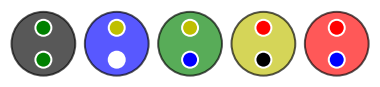
\includegraphics[scale= 0.45]{content/algo_bubble/modelization/example_a.png}
		
		[{\color{black} 2 , 2} , {\color{blue} $-1$ , 3} , {\color{ForestGreen} 1 , 3} , {\color{Goldenrod} 0 , 4} , {\color{red} 1 , 4}]


		\medskip     % [4, 2, 3, 0, 2, 3, 1, 4, 1, None]
		
		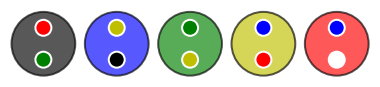
\includegraphics[scale= 0.45]{content/algo_bubble/modelization/example_b.png}
		
		[{\color{black} 2 , 4} , {\color{blue} 0 , 3} , {\color{ForestGreen} 2 , 3} , {\color{Goldenrod} 1 , 4} , {\color{red} $-1$ , 1}]
	\end{center}

	Les listes de nombres de même taille sont comparables comme le sont les mots d'un dictionnaire, on parle d'ordre lexicographique. Par exemple, nous avons :
	
	\medskip
	
	\begin{itemize}
		\item[\textbullet] $[\text{\color{red} \textbf{2} , \textbf{2} , \textbf{3}} \, , 1 \, , 3 \, , 0 \, , 4 \, , 1 \, , 4] > [\text{\color{red} \textbf{2} , \textbf{2} , \textbf{1}} \, , 3 \, , 0 \, , 4 \, , 1 \, , 3 \, , 4]$
		en comparant le $3$ et le $1$ aux troisièmes positions qui sont les premières valeurs à être différentes (par contre peu importe ce qu'il y a aux positions suivantes).

		\medskip

		\item[\textbullet] $[\text{\color{red} \textbf{1}} \, , 2 \, , 2 \, , 3 \, , 3 \, , 0 \, , 4 \, , 1 \, , 4] < [\text{\color{red} \textbf{2}} \, , 2 \, , 3 \, , 1 \, , 3 \, , 0 \, , 4 \, , 1 \, , 4]$
		en comparant le $1$ et le $2$ aux premières positions (sans se soucier des nombres qui suivent).
	\end{itemize}


	\medskip

	Nous n'allons pas comparer les deux listes $L(\mathscr{C}_1)$ et $L(\mathscr{C}_2)$ associées à deux configurations $\mathscr{C}_1$ et $\mathscr{C}_2$. Nous allons considérer à la place les sous-listes $SL(\mathscr{C}_1)$ et $SL(\mathscr{C}_2)$ obtenues en retirant le seul $(-1)$ présent dans les listes $L(\mathscr{C}_1)$ et $L(\mathscr{C}_2)$ respectivement (bien noter que les listes comparées via l'ordre lexicographique sont celles sans $(-1)$ la valeur du trou).
		
	
	\medskip

	Nous voilà armés pour faire notre démonstration sans encombre (mais pas sans réflexion).


	\medskip

	\textit{Fait n°1 : si le trou n'est pas dans la base n°0 alors les mouvements indiqués par l'algorithme amène le trou dans la base n°0.}


	\medskip
	
	C'est évident à condition d'avoir bien noté que pour la configuration gagnante, le trou est dans la base n°0.


	\medskip

	\textit{Fait n°2 : la configuration gagnante est la seule telle que le trou soit dans la base n°0 et telle que sa sous-liste soit minimale (c'est à dire qu'elle est inférieure ou égale à toutes les listes $SL(\mathscr{C})$ possibles).}


	\medskip

	Soit $\mathscr{G}$ la configuration gagnante. Il est clair que
	$SL(\mathscr{G}) = \text{[0 , 1 , 1 , 2 , 2 , \dots{} ]}$
	et que le trou est dans la base n°0.


	\medskip

	Soit $\mathscr{C}$ une configuration non gagnante. Si $SL(\mathscr{C}) \neq SL(\mathscr{G})$, il est évident que $SL(\mathscr{C}) > SL(\mathscr{G})$. Sinon si $SL(\mathscr{C}) = SL(\mathscr{G})$ c'est que le trou n'est pas dans la base n°0.
	
	
	\medskip

	\textit{Fait n°3 : lorsque l'un des mouvements demandés par l'algorithme est effectué, on passe d'une configuration $\mathscr{C}_1$ à une configuration $\mathscr{C}_2$. On a alors la relation : $SL(\mathscr{C}_2) \leqslant SL(\mathscr{C}_1)$.}


	\medskip

	Considérons le cas où le trou se déplace vers la droite. 
	Notons $L(\mathscr{C}_1) = [ \text{\ \dots{} , $-1$ , $x$ , $y$ , $z$ , \dots{} \ } ]$ où les points de suspension indiquent des éventuelles paires de valeurs.
	En particulier, $(-1)$ et $x$ sont les valeurs du trou et du jeton partageant la même base, tandis que $y$ et $z$ sont celles de deux autres jetons dans la base voisine à droite (notons que forcément $y \leqslant z$). Nous avons deux situations.

	\begin{enumerate}
		\item \textbf{Cas 1 :} $x \leqslant y$.
		
		Dans ce cas, $L(\mathscr{C}_2) = [ \text{\ \dots{} , $x$ , $y$ , $-1$ , $z$ , \dots{} \ } ]$ d'où $SL(\mathscr{C}_2) = SL(\mathscr{C}_1)$.
	
		\item \textbf{Cas 2 :} $y < x$.
		
		Dans ce cas, $L(\mathscr{C}_2) = [ \text{\ \dots{} , $y$ , $x$ , $-1$ , $z$ , \dots{} \ } ]$ d'où $SL(\mathscr{C}_2) < SL(\mathscr{C}_1)$.
		\end{enumerate}

	Le cas d'un déplacement vers la gauche se traite de façon analogue.
	
	
	\medskip

	\textit{Fait n°4 : si $\mathscr{C}$ est une configuration telle que $SL(\mathscr{C})$ ne soit pas minimale, l'algorithme fera apparaître à un moment ou à un autre une configuration $\mathscr{C}^\prime$ telle que $SL(\mathscr{C}^\prime) < SL(\mathscr{C})$ (en fait, le dit moment arrivera avant un éventuel aller-retour \quote{complet} du trou depuis sa base dans la configuration $\mathscr{C}$).}


	\medskip

	Comme $SL(\mathscr{C})$ n'est pas minimale, il existe au moins deux valeurs $x$ et $y$ telles que $x > y$ avec $y$ situé après $x$ dans $SL(\mathscr{C})$ lorsqu'on lit cette liste de gauche à droite. 
	La condition $x > y$ implique que $x$ et $y$ ne sont pas dans la même base. Nous avons : $L(\mathscr{C}) = [ \text{\ \dots{} , $x$ , \dots{} , $y$ , \dots{} \ } ]$ où les points de suspension indiquent d'éventuelles valeurs.


	\medskip
	
	Parmi tous les $y$ possibles, on choisit celui qui est le plus à gauche possible dans $SL(\mathscr{C})$, c'est à dire celui qui est le plus prêt de $x$ (dans ce cas, $y$ est la plus petite valeur de sa base).
	Avec ce choix, les valeurs éventuelles $w$ entre $x$ et $y$ dans $SL(\mathscr{C})$ vérifient toutes $y < x \leqslant w$. Ceci permet donc de choisir $x$ et $y$ voisins dans $SL(\mathscr{C})$ (avec des bases associés voisines différentes).
	Avec ce nouveau choix, $L(\mathscr{C}) = [ \text{\ \dots{} , $g$ , $x$ , $y$ , $d$ , \dots{} \ } ]$ où les points de suspension indiquent des éventuelles paires de valeurs. Notons que seul $g$ peut être égal à $(-1)$.
	Désignons par $\mathcal{B}_x$ et $\mathcal{B}_y$ les basses associées aux valeurs $x$ et $y$.
	
	
	\medskip
	
	Rappelons que tant que $SL(\mathscr{C})$ n'est pas minimale, la configuration $\mathscr{C}$ n'est pas une configuration gagnante et donc le trou se balade. Nous avons alors les situations suivantes.
	
	\begin{enumerate}
		\item \textbf{Cas 1 :} $g = -1$
		
		Si l'algorithme est dans une phase de déplacement vers la droite, alors comme dans la preuve du fait n°3, voir son cas 2, nous savons que la configuration suivante $\mathscr{C}^\prime$ vérifie $SL(\mathscr{C}^\prime) < SL(\mathscr{C})$ ce qui prouve ici le fait n°4.
		
		Sinon le trou va aller vers la base n°0. Si lors de ces déplacements, l'une des configurations $\mathscr{C}^\prime$ vérifie $SL(\mathscr{C}^\prime) < SL(\mathscr{C})$ alors le fait n°4 sera validé. Sinon le trou reviendra en direction de la base $\mathcal{B}_x$. Si lors de ces déplacements, l'une des configurations $\mathscr{C}^\prime$ vérifie $SL(\mathscr{C}^\prime) < SL(\mathscr{C})$ alors le fait n°4 sera validé. Sinon nous nous retrouvons dans le sous-cas traité ci-dessus où l'on avait un déplacement du trou vers la droite avec $g = -1$, et de nouveau nous obtenons le résultat souhaité.
		
		\item \textbf{Cas 2 :} $g \neq -1$ et le trou est à gauche de la base $\mathcal{B}_x$. 
		
		Si l'algorithme est dans une phase de déplacement vers la droite, alors le trou va prendre la place de $g$ et l'on retombe dans le cas 1. Si le déplacement se fait vers la gauche, on peut appliquer exactement le même raisonnement que dans le deuxième sous-cas du cas 1 traité ci-dessus.
		
		\item \textbf{Cas 3 :} $g \neq -1$ et le trou est à droite de la base $\mathcal{B}_y$. 
		
		L'algorithme va amener le trou dans la base voisine de $\mathcal{B}_y$ de sorte que l'on ait une configuration $\mathscr{C}^\prime$ telle que $L(\mathscr{C}^\prime) = [ \text{\ \dots{} , $g$ , $x$ , $y$ , $d$ , $-1$ , $\alpha$ , \dots{} \ } ]$ avec $SL(\mathscr{C}^\prime)$ non minimal.
		
		Si lors de ces déplacements une configuration $\mathscr{C}^{\prime\prime}$ vérifie $SL(\mathscr{C}^{\prime\prime}) < SL(\mathscr{C})$, le fait n°4 est bien entendu vérifié.
		Sinon $L(\mathscr{C}^\prime)$ devient $[ \text{\ \dots{} , $g$ , $x$ , $-1$ , $y$ , $?$ , $?$ , \dots{} \ } ]$, puis $[ \text{\ \dots{} , $-1$ , $g$ , {\color{red} $y$ , $x$} , $?$ , $?$ , \dots{} \ } ]$ où l'on utilisé le fait que $y < x$. Pour cette dernière liste, la configuration $\mathscr{C}^{\prime\prime\prime}$ vérifie $SL(\mathscr{C}^{\prime\prime\prime}) < SL(\mathscr{C})$ et c'est gagné !
	\end{enumerate}
	

	\medskip

	\textit{Finitude et résolution} : le fait n°1 nous permet de considérer le 1er moment où le trou est dans la base n°0.
	Si nous avons une configuration $\mathscr{C}$ gagnante, nous nous arrêtons comme demandé et il n'y a rien à prouver.


	\medskip
	
	Sinon la configuration $\mathscr{C}$  est telle que $SL(\mathscr{C})$ ne soit pas minimale d'après le fait n°2.
	Grâce au fait n°4, nous savons que nous arriverons ensuite à une configuration $\mathscr{C}^\prime$ telle que $SL(\mathscr{C}^\prime) < SL(\mathscr{C})$.
	Dès lors les faits n°3 et n°1 nous permettent d'affirmer que le trou va se retrouver dans base n°0 pour une configuration $\mathscr{C}^{\prime\prime}$ telle que $SL(\mathscr{C}^{\prime\prime}) \leqslant SL(\mathscr{C}^\prime) < SL(\mathscr{C})$. 


	\medskip
	
	En résumé, si le trou se retrouve dans la base n°0 pour une configuration $\mathscr{C}$ non gagnante, alors l'algorithme nous fera déplacer le trou jusqu'à le faire arriver de nouveau dans la base n°0 pour une nouvelle configuration $\mathscr{C}^{\prime\prime}$ telle que $SL(\mathscr{C}^{\prime\prime}) < SL(\mathscr{C})$.
	
	
	\medskip
	
	Pour conclure, il suffit de noter que le nombre de listes $SL(\mathscr{C})$ est fini.
	Dès lors il est impossible d'avoir une suite strictement décroissante de listes du type $SL(\mathscr{C})$.
	Ceci signifie que l'algorithme va en un nombre fini d'étapes amener le trou dans la base n°0 pour une configuration gagnante.  
\end{proof}


\paragraph{Remarque :} \hspace{-1em} la démonstration s'adapte sans problème à un nombre quelconque $n \geqslant 2$ de bases.


\section{À la recherche de solutions optimales}
	\subsection{Où tentons-nous d'aller ?}    % RELU. OK !
    	Commençons par noter que la méthode \quote{on avance au mieux} n'est pas la plus efficace possible comme le montre l'exemple suivant où six mouvements totalement inutiles sont effectués si bien que l'on n'a toujours pas gagné à la neuvième étape
\footnote{
    En fait, il faut $39$ mouvements pour gagner avec la méthode \quote{on avance au mieux}, et la méthode \quote{une base à la fois} en demande $25$.
}. Il est important de noter ici que nous appliquons à la lettre les mouvements demandés par l'algorithme ! Il est sûrement évident pour le lecteur de voir l'inutilité des tous premiers mouvements.

\vspace{-0.4em}
\begin{multicols}{2}
    \begin{center}   % [4, 4, None, 0, 1, 1, 2, 2, 3, 3]
        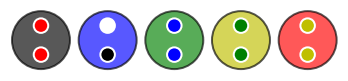
\includegraphics[scale= 0.45]{content/optimal/where_do_we_go/algo_bubble/000.png}

        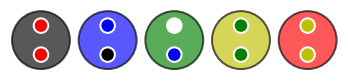
\includegraphics[scale= 0.45]{content/optimal/where_do_we_go/algo_bubble/001.png}

        
\includegraphics[scale= 0.45]{content/optimal/where_do_we_go/algo_bubble/002.png}

        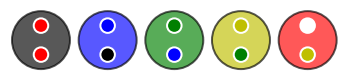
\includegraphics[scale= 0.45]{content/optimal/where_do_we_go/algo_bubble/003.png}

        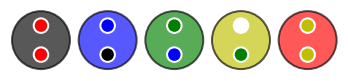
\includegraphics[scale= 0.45]{content/optimal/where_do_we_go/algo_bubble/004.png}
    \end{center}

    \columnbreak
    \begin{center}   % [4, 4, None, 0, 1, 1, 2, 2, 3, 3]
        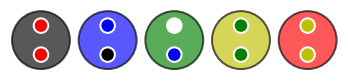
\includegraphics[scale= 0.45]{content/optimal/where_do_we_go/algo_bubble/005.png}

        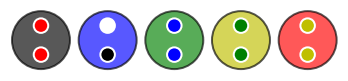
\includegraphics[scale= 0.45]{content/optimal/where_do_we_go/algo_bubble/006.png}

        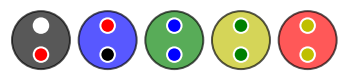
\includegraphics[scale= 0.45]{content/optimal/where_do_we_go/algo_bubble/007.png}

        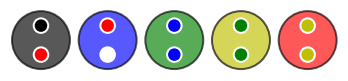
\includegraphics[scale= 0.45]{content/optimal/where_do_we_go/algo_bubble/008.png}

        \includegraphics[scale= 0.45]{content/optimal/where_do_we_go/algo_bubble/009.png}
    \end{center}
\end{multicols}


\medskip

Ici, on peut gagner en seulement 9 coups ! Voici les mouvements à faire
\footnote{
    Notez au passage les enseignements que l'on peut tirer d'une configuration très, très particulière.
}.
Nous verrons bientôt que l'on ne peut pas faire mieux.

\vspace{-0.4em}
\begin{multicols}{2}
    \begin{center}   % [4, 4, None, 0, 1, 1, 2, 2, 3, 3]
        \includegraphics[scale= 0.45]{content/optimal/where_do_we_go/tree_sol/000.png}

        \includegraphics[scale= 0.45]{content/optimal/where_do_we_go/tree_sol/001.png}

        \includegraphics[scale= 0.45]{content/optimal/where_do_we_go/tree_sol/002.png}

        \includegraphics[scale= 0.45]{content/optimal/where_do_we_go/tree_sol/003.png}

        \includegraphics[scale= 0.45]{content/optimal/where_do_we_go/tree_sol/004.png}
    \end{center}

    \columnbreak
    \begin{center}   % [4, 4, None, 0, 1, 1, 2, 2, 3, 3]
        \includegraphics[scale= 0.45]{content/optimal/where_do_we_go/tree_sol/005.png}

        \includegraphics[scale= 0.45]{content/optimal/where_do_we_go/tree_sol/006.png}

        \includegraphics[scale= 0.45]{content/optimal/where_do_we_go/tree_sol/007.png}

        \includegraphics[scale= 0.45]{content/optimal/where_do_we_go/tree_sol/008.png}

        \includegraphics[scale= 0.45]{content/optimal/where_do_we_go/tree_sol/009.png}
    \end{center}
\end{multicols}


\medskip

Précisions ce que nous cherchons à faire : nous voulons trouver une solution peu coûteuse. Très bien ! Mais dans ce cas, comment évalue-t-on ce coût ? Nous choisissons de chercher à minimiser le nombre de déplacements du trou (donc toute opération autre que le déplacement d'un jeton ne sera pas comptabilisée).
Dans le premier cas ci-dessus, le coût est strictement plus grand que $9$, tandis que pour le second, il vaut exactement $9$. La section suivante va proposer un algorithme donnant à coup sûr la solution la moins coûteuse.


	\subsection{La méthode \textit{\og tout connaître pour avancer vite \fg}}
    	Nous allons exploiter une idée toute simple à comprendre. Partons de la configuration gagnante pour trouver toutes les configurations obtenues en faisant un seul mouvement.
À partir des précédentes nouvelles configurations, nous recherchons ensuite d'autres configurations obtenues en faisant un second mouvement.
Ceci peut se résumer par l'arbre ci-dessous où une configuration $\mathcal{C}_1$ est reliée à une autre $\mathcal{C}_2$ uniquement si l'on peut passer de $\mathcal{C}_1$ à $\mathcal{C}_2$ en un seul mouvement. De plus, quand on descend dans l'arbre on ne garde que les nouvelles configurations.


\begin{center}
    \begin{tikzpicture}[
    rotate=0,
    level distance=1.5cm,
        level 1/.style={sibling distance=5cm},
        level 2/.style={sibling distance=2.25cm},
    ]
    \node{\includegraphics[scale=0.14]{content/optimal/tree_sol/moves/0.png}}
child{node{\includegraphics[scale=0.14]{content/optimal/tree_sol/moves/1.png}}
child{node{\includegraphics[scale=0.14]{content/optimal/tree_sol/moves/3.png}}}
child{node{\includegraphics[scale=0.14]{content/optimal/tree_sol/moves/4.png}}}}
child{node{\includegraphics[scale=0.14]{content/optimal/tree_sol/moves/2.png}}
child{node{\includegraphics[scale=0.14]{content/optimal/tree_sol/moves/5.png}}}
child{node{\includegraphics[scale=0.14]{content/optimal/tree_sol/moves/6.png}}}};
    \end{tikzpicture}
\end{center}



Avec un mouvement de plus, nous avons l'arbre ci-dessous (qui n'est pas symétrique : voir en bas à gauche).


\begin{center}
    \begin{tikzpicture}[
    rotate=0,
    level distance=1.5cm,
        level 1/.style={sibling distance=8.5cm},
        level 2/.style={sibling distance=4.75cm},
        level 3/.style={sibling distance=2cm},
    ]
    \node{\includegraphics[scale=0.12]{content/optimal/tree_sol/moves/0.png}}
child{node{\includegraphics[scale=0.12]{content/optimal/tree_sol/moves/1.png}}
child{node{\includegraphics[scale=0.12]{content/optimal/tree_sol/moves/3.png}}
child{node{\includegraphics[scale=0.12]{content/optimal/tree_sol/moves/7.png}}}
child{node{\includegraphics[scale=0.12]{content/optimal/tree_sol/moves/8.png}}}
child{node{\includegraphics[scale=0.12]{content/optimal/tree_sol/moves/9.png}}}}
child{node{\includegraphics[scale=0.12]{content/optimal/tree_sol/moves/4.png}}
child{node{\includegraphics[scale=0.12]{content/optimal/tree_sol/moves/10.png}}}
child{node{\includegraphics[scale=0.12]{content/optimal/tree_sol/moves/11.png}}}}}
child{node{\includegraphics[scale=0.12]{content/optimal/tree_sol/moves/2.png}}
child{node{\includegraphics[scale=0.12]{content/optimal/tree_sol/moves/5.png}}
child{node{\includegraphics[scale=0.12]{content/optimal/tree_sol/moves/12.png}}}
child{node{\includegraphics[scale=0.12]{content/optimal/tree_sol/moves/13.png}}}}
child{node{\includegraphics[scale=0.12]{content/optimal/tree_sol/moves/6.png}}
child{node{\includegraphics[scale=0.12]{content/optimal/tree_sol/moves/14.png}}}
child{node{\includegraphics[scale=0.12]{content/optimal/tree_sol/moves/15.png}}}}};
    \end{tikzpicture}
\end{center}



Avec de la patience, ou grâce à un programme, on peut fabriquer l'arbre complet (vous le trouverez en annexe). Notons que pour un jeu à cinq bases, il y a tout de même $11\,010$ configurations (ceci est justifié en annexe), donc représenter l'arbre complet pour 5 bases sur une feuille A3, même avec l'aide d'un programme, ne sera pas possible.


\medskip

Il est évident que la méthode que nous employons va finir par trouver toutes les configurations tout en nous indiquant une résolution proposant un minimum de coups à faire.
Il faut prendre garde que rien ne nous indique qu'il n'y a qu'une seule façon optimale de résoudre une configuration. En fait, il n'y a pas toujours unicité comme le montre la remarque n°1 juste après l'algorithme.


\medskip

Notre démarche peut se traduire par l'algorithme ci-dessous où nous utilisons des dictionnaires qui sont des objets associant une valeur à une clé. Par exemple, \verb+mon_dico = {"un": 1, "deux": 2}+ admet pour clés \verb+"un"+ et \verb+"deux"+, et nous notons \verb+mon_dico<"un"> = 1+ la valeur associée à la clé \verb+"un"+.
Nous utilisons aussi $[ \,\, ]$ pour indiquer une liste vide prête à être remplie.


\bigskip

\begin{algo}
    \Data{une configuration quelconque de début de jeu}
    \Result{la solution gagnante (en utilisant le moins de déplacements possible)}
    \vspace{0.4em}
    \Begin{
        \vspace{0.4em}
        $\cal G$ désigne la configuration gagnante.
        \\
        \vspace{0.4em}
        \tcp{"L'arbre" sera construit sous forme d'un dictionnaire.}
        \tcp{\quad \textbullet{} les clés sont les configurations possibles.}
        \tcp{\quad \textbullet{} chaque valeur donne la liste des configurations à suivre pour gagner}
        \tcp{\phantom{\quad \textbullet{}} le plus rapidement possible (lecture de la liste de gauche à droite).}
        $\mathcal{A} \leftarrow \{ \mathcal{G} : [ \,\, ] \}$
        \\
        \vspace{0.4em}
        \tcp{Liste stockant les [n]ouvelles [c]onfigurations d'où partir.}
        $NC \leftarrow \big[ \, \mathcal{G} \, \big]$
        \\
        \vspace{0.4em}
        \While{$NC$ n'est pas vide}{
            \vspace{0.4em}
            $NC_{ap} \leftarrow [ \,\, ]$ va stocker les configurations d'où partir durant l'étape d'après.
            \\
            \vspace{0.4em}
            \ForEach{configuration $\mathcal{C}$ dans $NC$}{
                \ForEach{configuration $\mathcal{V}$ obtenue en un seul mouvement depuis $\mathcal{C}$}{
                    \If{$\mathcal{V}$ n'est pas une clé de $\cal A$}{
                        \vspace{0.4em}
                        Ajouter $\mathcal{V}$ à $NC_{ap}$.
                        \\
                        \vspace{0.4em}
                        $COUPS$ : liste obtenue en ajoutant $\mathcal{C}$ à gauche de la liste $\mathcal{A} \big\langle \mathcal{C} \big\rangle$.
                        \\
                        Ajouter $\mathcal{V}$ à $\mathcal{A}$ avec $\mathcal{A} \big\langle \mathcal{V} \big\rangle = COUPS$.
                    }
                }
            }
            \vspace{0.4em}
            $NC \leftarrow NC_{ap}$
        }
        \vspace{0.4em}
        \tcp{Utilisation de l'arbre pour résoudre le jeu.}
        \vspace{0.4em}
        $\mathcal{C}_0$ : la configuration à résoudre.
        \\
        Obtenir successivement les configurations stockées de gauche à droite dans $\mathcal{A} \big\langle \mathcal{C}_0 \big\rangle$.
    }
\end{algo}


\medskip

\paragraph{Remarque n°1 :} \hspace{-1em} comme l'arbre construit  par l'algorithme \quote{tout connaître pour avancer vite} dépend de l'ordre dans lequel on explore les nouvelles possibilités, il y a peu de chances que l'on ait une solution optimale unique pour chaque configuration. L'exemple suivant montre qu'effectivement il n'y a pas unicité.

\vspace{-0.4em}
\begin{multicols}{2}
    \begin{center}   % [None, 0, 1, 2, 1, 2]
        \includegraphics[scale=0.25]{content/optimal/tree_sol/no_unicity/sol_1/000.png}

        \includegraphics[scale=0.25]{content/optimal/tree_sol/no_unicity/sol_1/001.png}

        \includegraphics[scale=0.25]{content/optimal/tree_sol/no_unicity/sol_1/002.png}

        \includegraphics[scale=0.25]{content/optimal/tree_sol/no_unicity/sol_1/003.png}
    \end{center}

    \columnbreak
    \begin{center}   % SAME START
        \includegraphics[scale=0.25]{content/optimal/tree_sol/no_unicity/sol_1/000.png}

                     % [1, 0, 1, 2, None, 2]
        \includegraphics[scale=0.25]{content/optimal/tree_sol/no_unicity/sol_2/001.png}

                     % [1, 0, 1, None, 2, 2]
        \includegraphics[scale=0.25]{content/optimal/tree_sol/no_unicity/sol_2/002.png}

                     % SAME END
        \includegraphics[scale=0.25]{content/optimal/tree_sol/no_unicity/sol_1/003.png}
    \end{center}
\end{multicols}

Ceci étant noté, si l'on visualise le jeu en cercle, et non plus en ligne, les deux solutions précédentes sont équivalentes puisque sur chaque ligne, la configuration de gauche et celle de droite sont dans le cercle symétriques par rapport à la base noire.
Autrement dit, la colonne de droite est obtenue à partir de celle de gauche en échangeant les couleurs rouges et jaunes, et aussi l'ordre des deux bases rouges et jaunes (ce qui est autorisé puisque l'on choisit un sens de parcours pour \quote{aplatir} le cercle).

\paragraph{Remarque n°2 :} \hspace{-1em} si l'on considère l'exemple donné dans la section précédente \quote{Où tentons-nous d'aller ?}, la méthode \quote{tout connaître pour avancer vite} propose exactement les 9 coups proposés pour illustrer certaines maladresses de l'algorithme \quote{on avance au mieux}


\paragraph{Remarque n°3 :} \hspace{-1em} l'algorithme \quote{tout connaître pour avancer vite}, bien que facile à programmer, est inutilisable par un humain dès le jeu à quatre bases qui permet d'avoir $480$ configurations différentes (voir l'annexe pour le calcul de cette valeur).
    % RELU ? NON

%	\subsection{La méthode du \textit{\og flemmard calculateur \fg}}
%    	??????

on change de démarche, on s'appuie sur l'arbre pour essayer de valider une intuition consistant à toujours chercher à obtenir une liste plus petite etc...

duc coup on produit un arbre faisant apparaître SL : ici on n'utuilise plus tikz mais on passe via dirtree TOP !!!!    % RELU ? NON



\clearpage

\section{Annexe}
	\subsection{Toutes les configurations pour un jeu à trois bases}    % RELU. OK !
	    L'arbre ci-dessous
\footnote{
	Bien entendu, cet arbre a été obtenu via un programme et non à la main.
}
permet de gagner en un minimum de coups au baseball des couleurs pour trois bases (il y a 33 configurations différentes et dans le pire des cas on peut gagner en cinq coups).
Pour cela, repérer la configuration à résoudre puis suivre les arêtes de la droite vers la gauche pour avoir les mouvements à faire.


\begin{center}
    \begin{tikzpicture}[
    rotate=90,
    level distance=2.5cm,
        level 1/.style={sibling distance=10cm},
        level 2/.style={sibling distance=5cm},
        level 3/.style={sibling distance=2cm},
        level 4/.style={sibling distance=1cm},
        level 5/.style={sibling distance=0.5cm},
    ]
    \node{\includegraphics[scale=0.12]{content/optimal/tree_sol/moves/0.png}}
child{node{\includegraphics[scale=0.12]{content/optimal/tree_sol/moves/1.png}}
child{node{\includegraphics[scale=0.12]{content/optimal/tree_sol/moves/3.png}}
child{node{\includegraphics[scale=0.12]{content/optimal/tree_sol/moves/7.png}}
child{node{\includegraphics[scale=0.12]{content/optimal/tree_sol/moves/16.png}}
child{node{\includegraphics[scale=0.12]{content/optimal/tree_sol/moves/26.png}}}}
child{node{\includegraphics[scale=0.12]{content/optimal/tree_sol/moves/17.png}}
child{node{\includegraphics[scale=0.12]{content/optimal/tree_sol/moves/27.png}}}}}
child{node{\includegraphics[scale=0.12]{content/optimal/tree_sol/moves/8.png}}}
child{node{\includegraphics[scale=0.12]{content/optimal/tree_sol/moves/9.png}}
child{node{\includegraphics[scale=0.12]{content/optimal/tree_sol/moves/18.png}}
child{node{\includegraphics[scale=0.12]{content/optimal/tree_sol/moves/28.png}}}
child{node{\includegraphics[scale=0.12]{content/optimal/tree_sol/moves/29.png}}}}
child{node{\includegraphics[scale=0.12]{content/optimal/tree_sol/moves/19.png}}
child{node{\includegraphics[scale=0.12]{content/optimal/tree_sol/moves/30.png}}}}}}
child{node{\includegraphics[scale=0.12]{content/optimal/tree_sol/moves/4.png}}
child{node{\includegraphics[scale=0.12]{content/optimal/tree_sol/moves/10.png}}
child{node{\includegraphics[scale=0.12]{content/optimal/tree_sol/moves/20.png}}}}
child{node{\includegraphics[scale=0.12]{content/optimal/tree_sol/moves/11.png}}
child{node{\includegraphics[scale=0.12]{content/optimal/tree_sol/moves/21.png}}}}}}
child{node{\includegraphics[scale=0.12]{content/optimal/tree_sol/moves/2.png}}
child{node{\includegraphics[scale=0.12]{content/optimal/tree_sol/moves/5.png}}
child{node{\includegraphics[scale=0.12]{content/optimal/tree_sol/moves/12.png}}}
child{node{\includegraphics[scale=0.12]{content/optimal/tree_sol/moves/13.png}}
child{node{\includegraphics[scale=0.12]{content/optimal/tree_sol/moves/22.png}}}}}
child{node{\includegraphics[scale=0.12]{content/optimal/tree_sol/moves/6.png}}
child{node{\includegraphics[scale=0.12]{content/optimal/tree_sol/moves/14.png}}
child{node{\includegraphics[scale=0.12]{content/optimal/tree_sol/moves/23.png}}}
child{node{\includegraphics[scale=0.12]{content/optimal/tree_sol/moves/24.png}}
child{node{\includegraphics[scale=0.12]{content/optimal/tree_sol/moves/31.png}}}}}
child{node{\includegraphics[scale=0.12]{content/optimal/tree_sol/moves/15.png}}
child{node{\includegraphics[scale=0.12]{content/optimal/tree_sol/moves/25.png}}
child{node{\includegraphics[scale=0.12]{content/optimal/tree_sol/moves/32.png}}}}}}};
    \end{tikzpicture}
\end{center}




	\subsection{Calculer le nombre de configurations possibles}    % RELU. OK !
	    On peut se demander combien de configurations de jeux sont possibles. C'est ce que nous allons chercher à calculer. Soit $C(n)$ le nombre de configurations de jeux pour $n \geqslant 1$ base(s) (par exemple, $C(1) = 1$). Nous avons au total $(2n - 1)$ jetons et $n$ \quote{couleurs} différentes.
Nous dirons que le jeton associé au trou est le jeton noir. 
Enfin, nous allons noter $\mathcal{B}_1$ , $\mathcal{B}_2$ , \dots{} , et  $\mathcal{B}_n$ les bases \quote{rangées} dans l'ordre initial de mise en place du jeu. Dans la suite, nous supposerons $n \geqslant 2$.


\medskip

Commençons par examiner les configurations telles que la base $\mathcal{B}_1$ contienne le trou. Nous avons alors deux situations
\footnote{
	Le lecteur notera que ce qui compte dans les raisonnements de cette section, c'est la couleur tirée et non le jeton tiré. C'est une subtilité importante à noter.
	Dans une première version de ce document, l'auteur avait raisonné sur les jetons, ce qui lui avait fait obtenir et \quote{démontrer} une formule fausse.
	Cette erreur a été repérée très rapidement lors de la fabrication de l'arbre présenté dans la section précédente.
}.

\begin{enumerate}
    \item \textit{$\mathcal{B}_1$ contient aussi le jeton noir.} 
    Dans ce cas, nous devons compter le nombre de façons différentes de placer des jetons à partir de $(n - 1)$ paires de jetons de même couleur sur $(n-1)$ bases, sachant que sur chaque base l'ordre des jetons n'est pas important. Nous n'allons pas chercher à calculer ce nombre. Nous le notons juste $P(n - 1)$ (les hypothèses sur les couleurs sont similaires à celles du jeu du baseball des couleurs sauf que l'on n'a plus de trou, ni de jeton noir associé au trou). Indiquons que l'on a clairement $P(1) = 1$.
        
    \item \textit{$\mathcal{B}_1$ ne contient pas le jeton noir.} 
    Notant $c$ la couleur du jeton dans la base $\mathcal{B}_1$, sur les $(n-1)$ bases restantes, il reste à placer $(n - 2)$ paires de jetons de même couleur, ainsi que deux jetons de couleurs différentes \quote{sans jumeau}, à savoir les jetons de couleurs respectives $c$ et noire. Interprétant le jeton de couleur $c$ comme un trou, nous retombons sur une configuration d'un jeu de baseball des couleurs mais avec $(n-1)$ jetons. Ceci nous fait donc $C(n -1)$ possibilités associées à la couleur $c$. 
\end{enumerate}

D'après ce qui précède, il y a donc $P(n - 1) + (n-1) C(n-1)$ configurations possibles telles que la base $\mathcal{B}_1$ contienne le trou. Dans $(n-1) C(n-1)$, le \quote{fois $(n-1)$} vient de ce que l'on a $(n-1)$ choix possibles pour la couleur $c$.


\medskip

En répétant le raisonnement précédent, et en notant qu'il y a $n$ choix de bases où placer le trou, nous arrivons à la relation $C(n) = n \left[ P(n - 1) + (n-1) C(n-1) \right]$. Nous réécrivons ceci comme suit :
\begin{equation}
    C(n) = n P(n - 1) + n(n-1) C(n-1)
\end{equation}


Nous allons reprendre un raisonnement similaire à ce qui a été fait ci-dessus pour trouver une relation de récurrence pour tenter d'évaluer $P(n)$ le nombre de façons de placer des jetons à partir de $n$ paires monochromes de jetons sur $n$ bases
\footnote{
   Il y a autant de couleurs différentes que de bases.
}.
De nouveau, nous allons d'abord raisonner sur la base $\mathcal{B}_1$. Deux cas sont possibles.

\begin{enumerate}
    \item \textit{$\mathcal{B}_1$ contient deux jetons de la même couleur $c$.}
    Dans ce cas, il y a $P(n - 1)$ possibilités de placer les autres jetons sur les bases restantes. En effet, on a enlevé une paire monochrome de couleur $c$ et la base $\mathcal{B}_1$ de couleur $d$. Si $c = d$, l'affirmation est évidente, sinon il suffit d'associer la couleur de jeton $d$ à la couleur de base $c$ pour les bases et les jetons restants.
        
    \item \textit{$\mathcal{B}_1$ contient deux jetons de couleurs différentes $c_1$ et $c_2$.}
    Dans les jetons restants, il y a juste deux jetons sans \quote{jumeau}, à savoir ceux de couleurs $c_1$ et $c_2$. Interprétant $c_1$ comme étant la \quote{couleur} du trou, et $c_2$ celle du jeton associé au trou, nous avons alors une configuration de type baseball des couleurs pour les jetons et les bases restants. Nous avons donc $C(n - 1)$ possibilités dans ce cas.
\end{enumerate}


\medskip

Dans le premier cas, pour la base $\mathcal{B}_1$, il y a $n$ choix de couleurs, ce qui nous fait $n P(n - 1)$ configurations avec une première base monochrome.
Dans le second cas, pour la base $\mathcal{B}_1$ nous avons $n$ choix pour la première couleur, et $(n - 1)$ pour la seconde (car l'on veut deux couleurs différentes).
Comme l'ordre ne compte pas, car tirer $c_1$ puis $c_2$, ou bien tirer $c_2$ puis $c_1$ nous donne à chaque fois la même base complétée, nous avons donc $\frac{n(n - 1)}{2}$ façons de remplir la première base avec deux couleurs différentes.
Nous en déduisons que nous avons $\frac{n(n-1)}{2} C(n - 1)$ configurations avec une première base non monochrome.
Nous arrivons finalement à la relation suivante.
\begin{equation}
    P(n) = n P(n - 1) + \dfrac{n(n-1)}{2} C(n - 1)
\end{equation}


En résumé, nous avons démontré les deux relations de récurrence suivantes pour $n \in \NN^* - \{1\}$ avec les conditions initiales $C(1) = P(1) = 1$ :
\begin{equation}
	\begin{cases}
		C(n) = n P(n - 1) + n(n-1) C(n-1) \\
		P(n) = n P(n - 1) + \dfrac{n(n-1)}{2} C(n - 1)
	\end{cases}
\end{equation}


\medskip

Ceci n'est pas très difficile à programmer. En utilisant le logiciel SageMath directement en ligne à l'adresse suivante \url{https://sagecell.sagemath.org}, il suffit d'insérer le code de type Python suivant.


\bigskip

\begin{myverb}
def C(n):
    if n == 1:
        return 1
        
    return n * P(n - 1) + n*(n-1)*C(n - 1)


def P(n):
    if n == 1:
        return 1
        
    return n * P(n - 1) + n*(n-1)/2*C(n - 1)

       
for k in range(2, 6):
    print "Pour k =", k, ":", C(k)

\end{myverb}

\bigskip

Ceci nous donne les résultats suivants.

\medskip

\begin{itemize}
    \item[\textbullet] $C(2) = 4$ ce qui est calculable directement en imaginant les configurations possibles avec deux bases.

    \medskip

    \item[\textbullet] $C(3) = 33$,
                       $C(4) = 480$ et
                       $C(5) = 11\,010$.
\end{itemize}


\medskip

Par contre, si l'on veut par exemple calculer $C(36)$, il faut être un peu plus précautionneux car dans le code précédent certains calculs sont effectués plusieurs fois. Le code suivant permet d'obtenir instantanément $C(36)$ alors que celui ci-dessus fait ceci très, très, très lentement... L'astuce consiste à stocker tout ce qui est calculé et de regarder si une valeur à calculer a déjà été stockée en mémoire. Si c'est le cas, on récupère directement cette valeur, sinon on la calcule et on la stocke en mémoire en vue d'éventuelles utilisations à venir (nous faisons ceci \quote{à la main} en utilisant des dictionnaires Python).

\bigskip

\begin{myverb}
valsP, valsC = \{\}, \{\}


def C(n):
    if n == 1:
        return 1
        
    global valsC
    
    if n in valsC:
        return valsC[n]

    val      = n * P(n - 1) + n*(n-1)*C(n - 1)  
    valsC[n] = val
    
    return val


def P(n):
    if n == 1:
        return 1

    global valsP
    
    if n in valsP:
        return valsP[n]

    val      = n * P(n - 1) + n*(n-1)/2*C(n - 1)
    valsP[n] = val
    
    return val

  
print C(36).n(10)

\end{myverb}

\bigskip

Ceci nous donne, sans temps de latence, $C(36) \approx 4,\!2 \times 10^{82}$ que l'on comparera à $10^{80}$ qui est une estimation du nombre d'atomes dans l'univers
\footnote{
    Notons que si l'estimation du nombre d'atomes de l'univers est juste, alors il est tout simplement impossible \quote{d'écrire} tous les naturels de $1$ à $C(36)$ en associant chaque naturel à un seul atome de l'univers. Vertigineux !
}.


\end{document}
